\section{Design di dettaglio}
Design di dettaglio (scelte rilevanti, pattern di progettazione, organizzazione del codice -- corredato da pochi ma efficaci diagrammi)
Di seguito verranno analizzate le scelte di design rilevanti per il sistema, i pattern di progettazione utilizzati e l'organizzazione del codice. 
\subsection{GameModel}
L'intero modello di gioco, dallo stato al comportamento, è incapsulato all'interno della struttura GameModel. E' possibile identificare due diverse accezioni del modello, a seconda del momento di gioco. 
Un momento in cui la partita non è ancora stata avviata e un momento successivo in cui invece la partita è avviata.
Nel primo momento, a partita non avviata, è necessario generare il dungeon e le stanze che lo compongono. Nel secondo momento, una volta che è avvenuta la generazione, il modello è costituito da un Dungeon, composto da diverse stanze, e dal character controllato dal giocatore. 

\begin{figure}[!hbt]
    \centering
    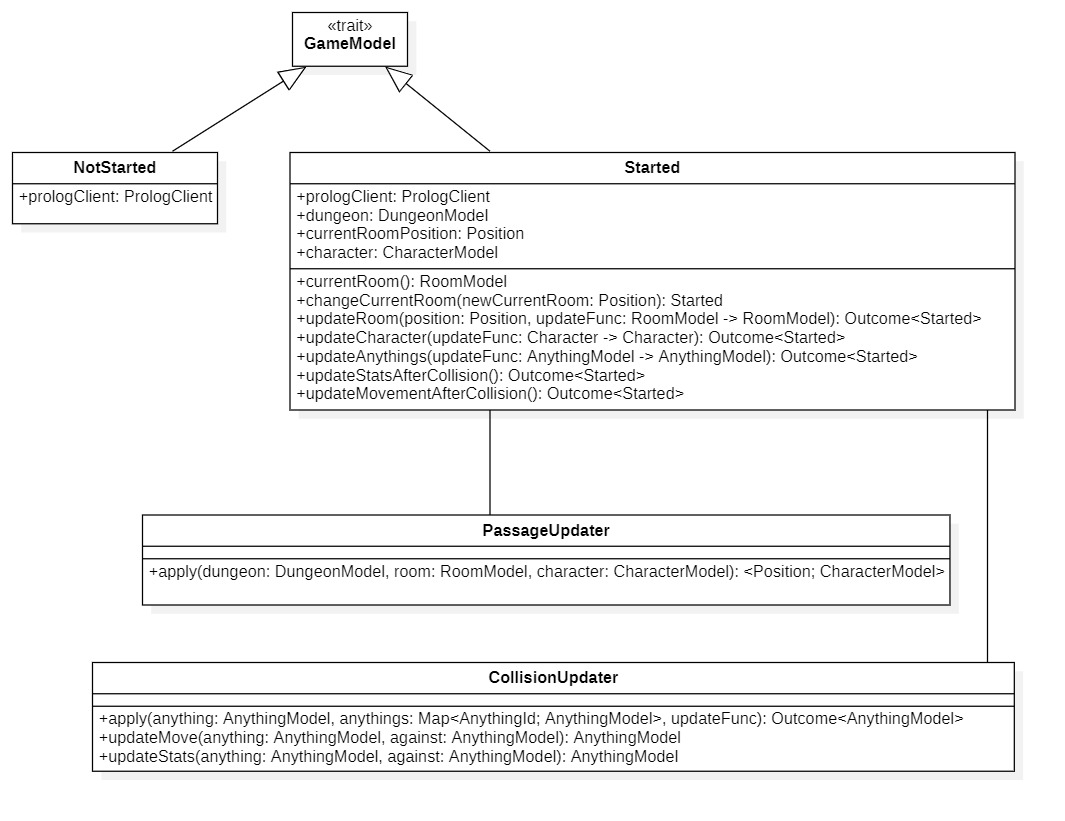
\includegraphics[scale=0.2]{GameModelClassDiagram.jpg}
    \caption{\textit{Game model class diagram (da modificare con versione pro di staruml)}} 
\end{figure}
Il modello di gioco rappresenta un'istantanea delle varie componenti che lo compongono in un determinato momento. 
Ogni modifica al modello consiste nella creazione di un nuovo modello con il componente aggiornato. 

Una scelta rilevante ai fini dell'implementazione è il fatto che, a livello di modello, il character controllato dal giocatore è sempre fuori dalla stanza in cui si trova, in questo modo è possibile aggiornare in maniera indipendente le due componenti.
\subsection{Dungeon}
Il dungeon è composto da stanze disposte in maniera randomica ma collegate tra loro. 
La struttura Grid è ciò che descrive un Dungeon nella sua forma più basilare e geometrica e offre delle operazioni per esplorarlo. 
\begin{figure}[!hbt]
    \centering
    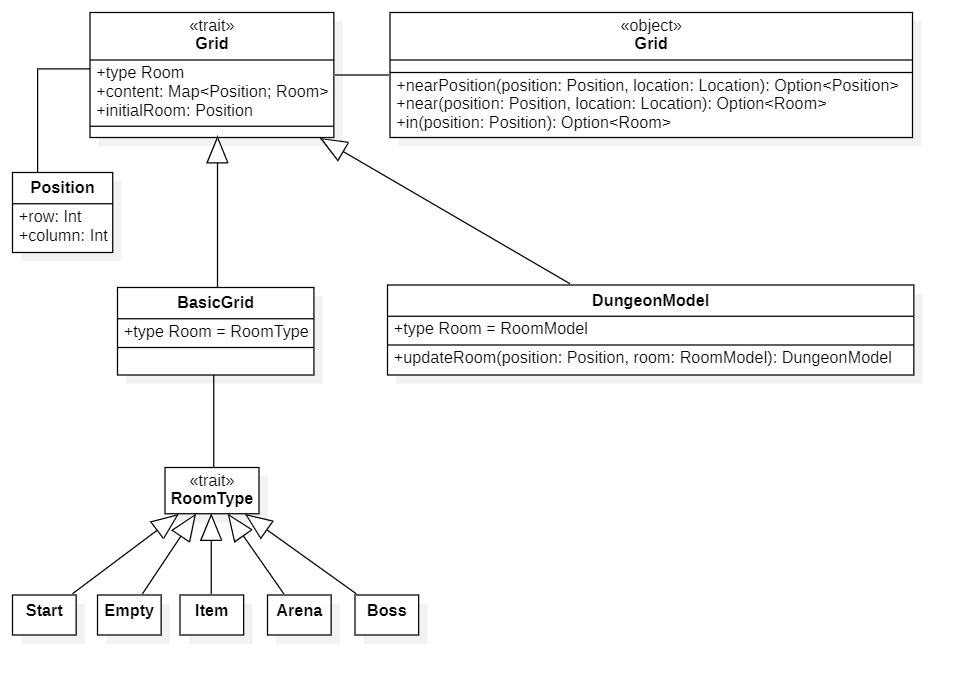
\includegraphics[scale=0.2]{DungeonClassDiagram.jpg}
    \caption{\textit{Dungeon class diagram(da modificare con versione pro di staruml)}} 
\end{figure}

Grid definisce quindi una collezione di stanze, di tipo ancora non definito, in una specifica posizione all'interno di una griglia di dimensioni \textit{n}. La definizione del tipo Room è lasciato alle specializzazioni di Grid, si mette quindi in pratica il pattern \textbf{Family Polimorfism}.

All'interno di una griglia, un elemento potrebbe o non potrebbe essere presente, andando così a definire un dungeon con stanze in posizioni diverse. 
E' necessario perciò lavorare con strutture dati che consentano l'assenza di un dato.

Il Dungeon vero e proprio prende forma quando il tipo Room viene definito con un modello consono a descriverne lo stato e il comportamento. 

\subsection{Room}
Come da requisiti, una stanza è la componente principale del Dungeon e può essere di diversi tipi: Empty, Arena, Item e Boss. 
Ogni stanza incapsula al suo interno gli elementi che sono rilegati all'interno e non possono muoversi all'interno del Dungeon, come ad esempio i nemici o gli elementi bloccanti. 

\begin{figure}[!hbt]
    \centering
    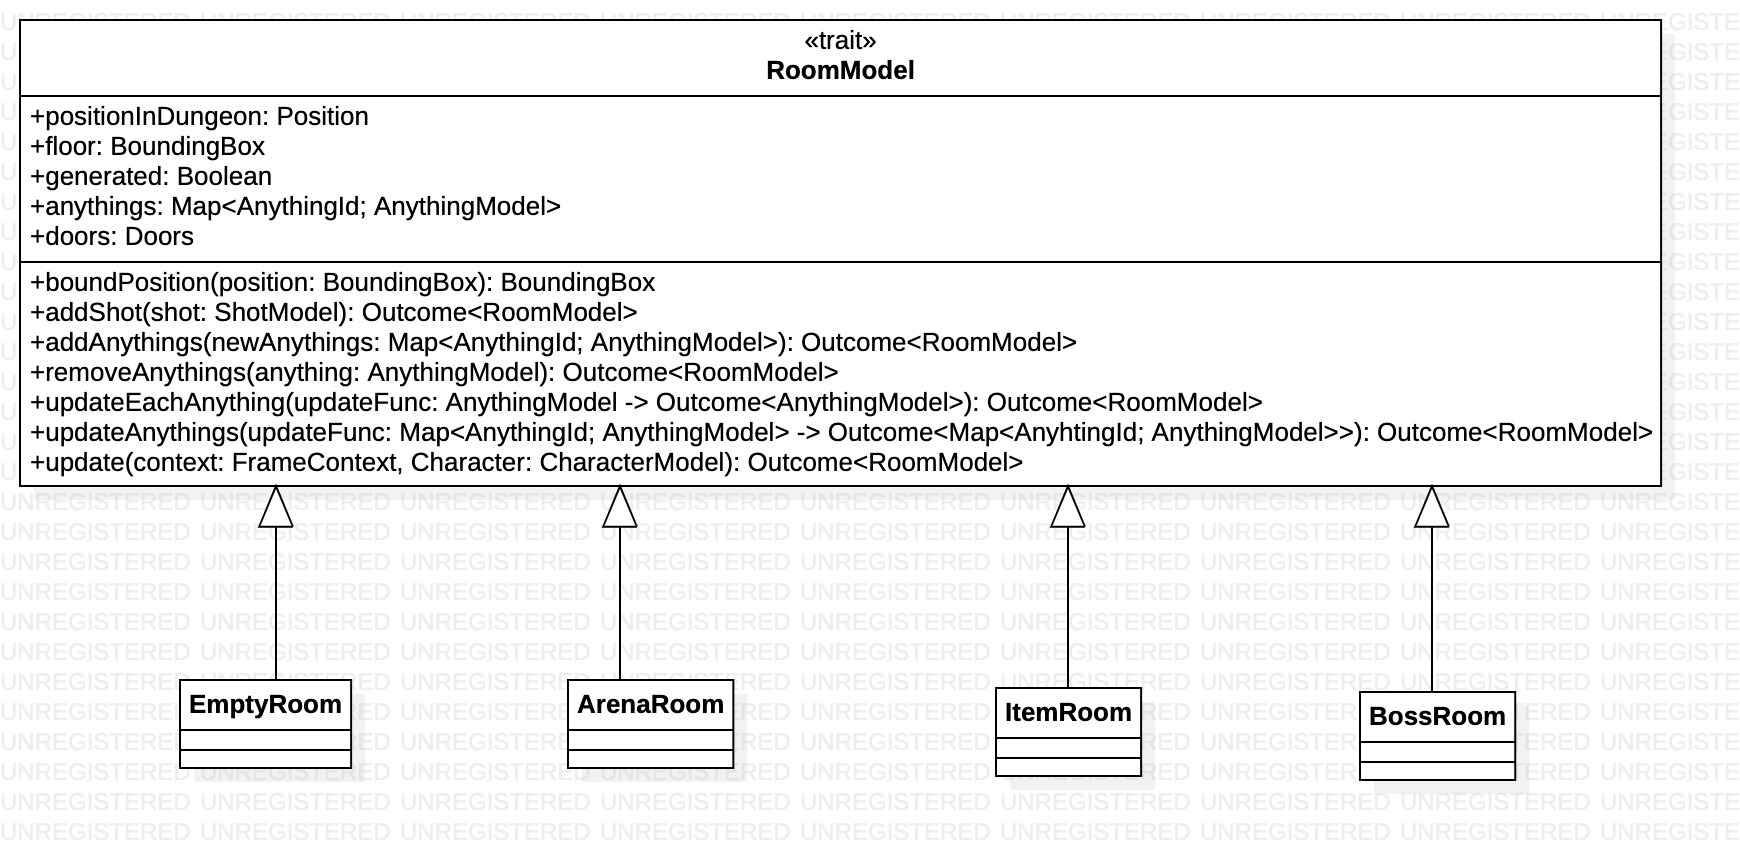
\includegraphics[scale=0.25]{RoomClassDiagram.jpg}
    \caption{\textit{Room class diagram(da modificare con versione pro di staruml)}} 
\end{figure}

Una stanza è anche responsabile dell'aggiornamento di tutto ciò che incapsula. Anche in questo caso si cerca di lavorare con strutture dati immutabili, perciò l'aggiornamento di uno o più componenti consegue una nuova stanza aggiornata. 
L'aggiornamento viene fatto ad ogni FrameTick ed è comandato dal dungeon, solamente per la stanza correntemente visualizzata, le altre stanze non sono aggiornate o gestite.  

\subsubsection{Door}
Un dettaglio importante di una stanza sono le porte che la collegano con altre stanze. Si è scelto di definire una porta non tanto come un link, ma come una proprietà statica, lasciando al Dungeon il compito di gestire il collegamento. 
Una porta è quindi l'associazione di un lato della stanza con lo stato della stessa. Il fatto che vi sia una porta, presuppone comunque che dalla parte opposta vi sia un'altra stanza, ma questo dettaglio è trasparente alla stanza e gestita dal Dungeon. 
\begin{figure}[!hbt]
    \centering
    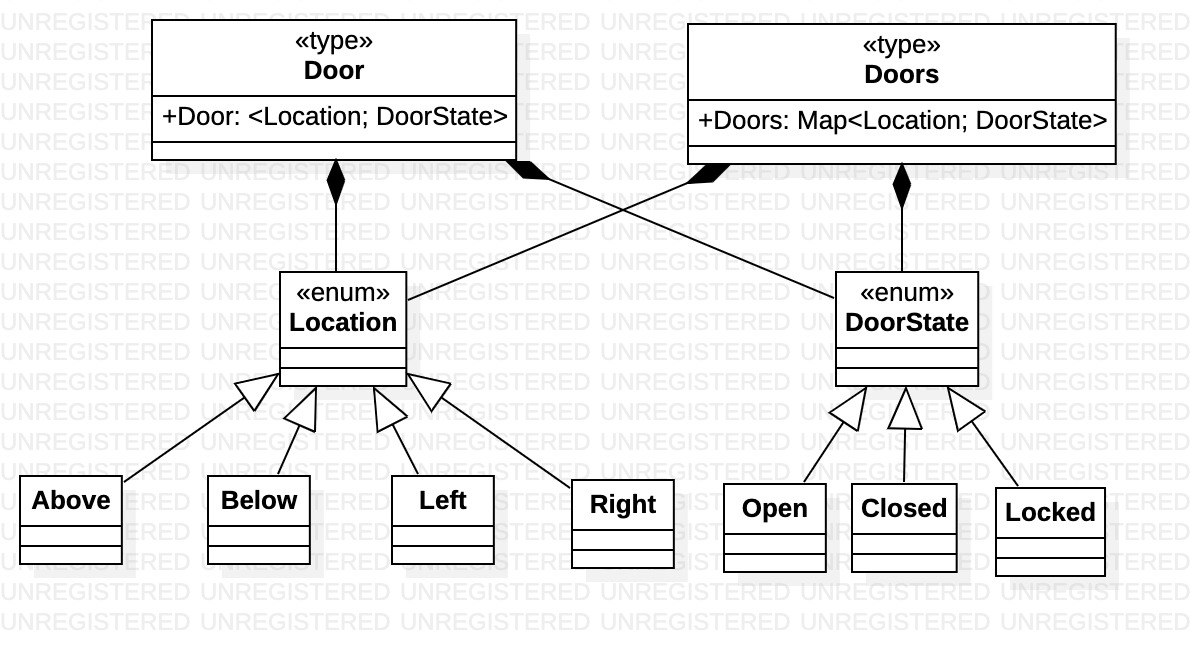
\includegraphics[scale=0.25]{DoorClassDiagram.jpg}
    \caption{\textit{Door class diagram(da modificare con versione pro di staruml)}} 
\end{figure}

\subsection{AnythingModel}
In generale ogni oggetto in gioco contiene un identificativo univoco e una bounding box che ne determina posizione e dimensioni 2D, inoltre ad ogni istanza è associata la factory per la sua View in modo tale che, quando una collezione di AnythingModel viene renderizzata, è sufficiente creare la View e chiamare il metodo draw. 

Ogni oggetto inoltre reagisce alla richiesta di update che avviene ad ogni iterazione del game loop, ma il modo con cui lo fa dipende da specifici comportamenti definiti come sottotipi mixabili di AnythingModel.

I sottotipi principali sono:
\begin{itemize}
    \item \textbf{DynamicModel} un oggetto in grado di spostarsi autonomamente durante un update, dove e come viene stabilito dalla classe che esegue il mixing attraverso l'implementazione di alcuni template-method predisposti
    \item \textbf{AliveModel} un oggetto vivo che può essere colpito perdendo vita. Non ha comportamento autonomo.
    \item \textbf{DamageModel} un oggetto che provoca danno di contatto. Non ha comportamento autonomo.
    \item \textbf{FireModel} un oggetto in grado di sparare autonomamente durante un update, dove e come viene stabilito dalla classe che esegue il mixing attraverso l'implementazione di alcuni template-method predisposti. Durante l'update può emettere uno ShotEvent contenente ShotModel
    \item \textbf{SolidModel} un oggetto solido che non può essere fisicamente attraversato da un altro. Non ha comportamento autonomo.
\end{itemize}

Questi tratti possono richiedere delle Stats per ottenere dei parametri al loro funzionamento (ad esempio la velocità massima da applicare ad uno spostamento): le Stats se richieste sono assegnate durante l'istanzazione di un Model ma possono cambiare durante il gioco.

Di seguito in figura 10 mostriamo un estratto della gerarchia di AnythingModel con tutti i sottotipi che aggiungono proprietà e comportamenti al Model di base e che possono essere estesi o mixati da un Model finale.

\begin{figure}[!hbt]
    \centering
    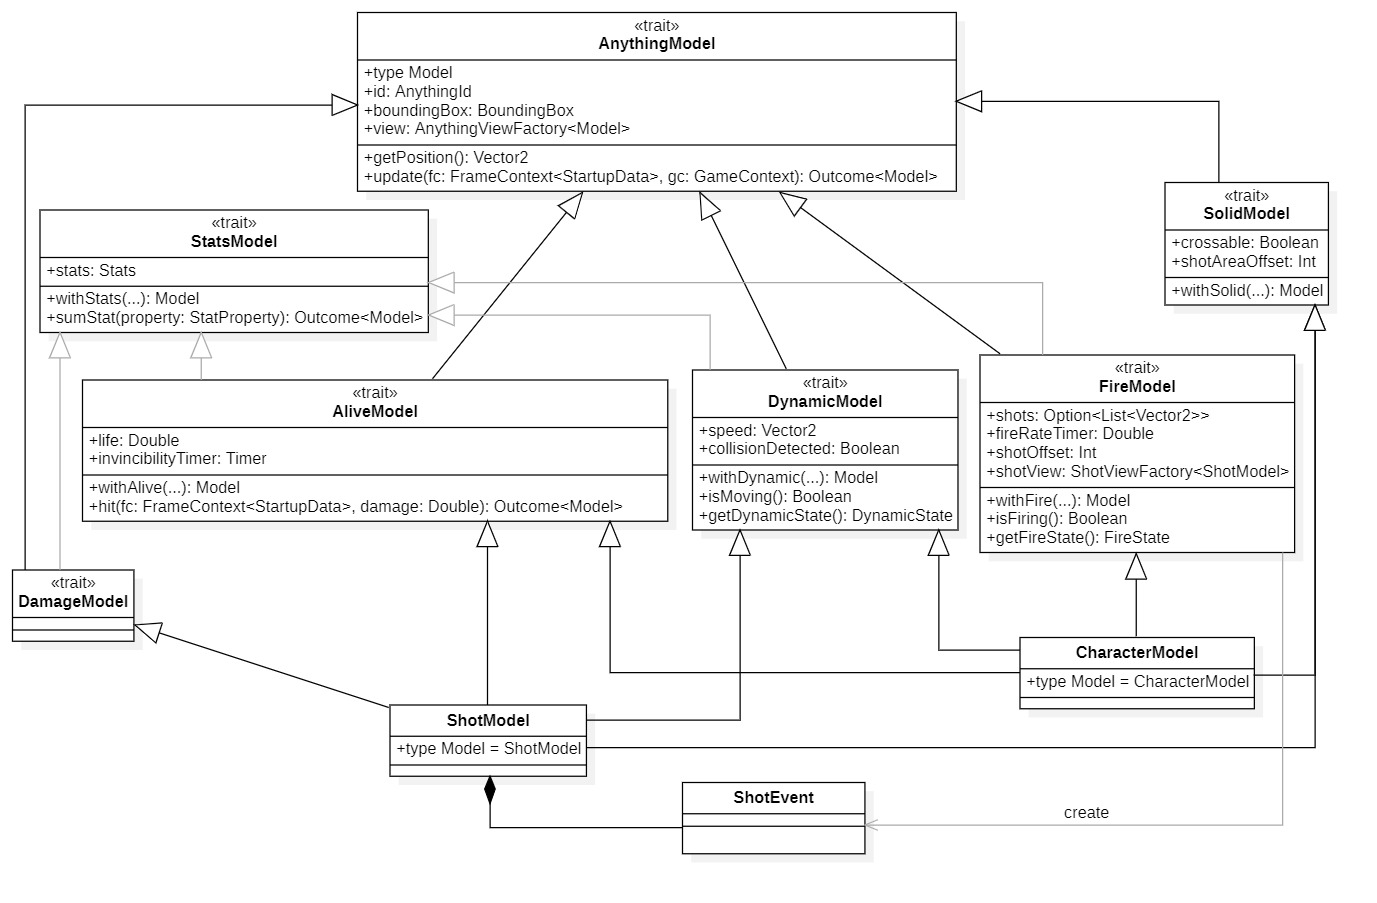
\includegraphics[scale=0.37]{AnythingModel.jpg}
    \caption{\textit{Gerarchia AnythingModel}} 
\end{figure}

\subsubsection{Update e immutabilità}

Ogni metodo che applica modifica al Model, a partire da update che viene richiamata ad ogni iterazione del game loop, deve ritornare una \textbf{copia aggiornata} dello stesso e del \textbf{tipo corrente}: adottiamo il pattern \textbf{F-Bounded Polymorphism con type-member}. 
Allo scopo predisponiamo un type member astratto Model e per ogni trait un template method with***(...) che accetta come argomenti quelli da modificare e ritorna un nuovo oggetto aggiornato di tipo Model: entrambi da definire nella classe finale che mixa il trait.
E' richiesto che il metodo update richiami super.update in modo da propagare l'aggiornamento a tutti i trait mixati.
\textit{Si rimanda all'implementazione per il dettaglio di come il pattern viene applicato con Scala.}

Per concludere, il metodo update riceve in input, oltre al FrameContext di Indigo, il \textbf{GameContext} che contiene lo stato della stanza corrente e il CharacterModel in modo da permettere all'oggetto in gioco comportamenti che si adattano alla situazione.

\paragraph{Nota} Sebbene una soluzione consigliata in sostituzione al polimorfismo F-Bounded è quella di impiegare polimorfismo ad-hoc con typeclass, abbiamo riscontrato che nel nostro caso volendo mantenere il mixing degli oggetti questo pattern non è facilmente applicabile e avrebbe generato più boilerplate code.

\paragraph{Nota}
Abbiamo deciso di inglobare il comportamento nei Model con il metodo update, ma un alternativa forse migliore e più semplice era delegarlo a sistemi esterni, i quali si sarebbero occupati ad esempio di spostare gli oggetti, farli sparare, etc: in questo progetto abbiamo cercato di emulare un modello ad agenti oltre che garantirci la massima possibilità di personalizzazione del comportamento soprattutto per quanto riguarda i nemici. 

\subsubsection{Gestione degli spari}
Riguardo a FireModel e agli spari \textbf{ShotModel} occorre specificare che:
\begin{itemize}
    \item possono essere sparati più colpi ShotModel contemporaneamente in direzioni diverse
    \item tra un colpo e l'altro deve trascorrere del tempo in base alla Stats "rate di fuoco"
    \item occorre generare il colpo a certo un offset rispetto alla posizione del oggetto che sta separando
    \item occorre specificare una ShotView factory da passare allo ShotModel, infatti in questo caso sono disponibili più View da utilizzare
\end{itemize}
FireModel durante un update genera l'evento \textbf{ShotEvent} indicando le proprietà dello ShotModel da istanziare (tra cui velocità e danno) ed inserendolo nella monade Outcome di ritorno: verrà gestito nell'iterazione successiva del game loop e aggiunto al RoomModel.

\subsubsection{Mini framework per i nemici}

Abbiamo pensato ad un mini framework che consenta la creazione rapida di nuovi nemici in modo da soddisfare i requisiti di possibili future espansioni.
Al centro abbiamo \textbf{EnemyModel}, il quale dispone di una coda di stati temporizzati che vengono processati uno dopo l'altro: questo permette la realizzazione di nemici che eseguono una sequenza di azioni.
Sono stati definiti dei comportamenti mixabili elementari come:
\begin{itemize}
    \item \textbf{Follower}: un nemico che insegue il character
    \item \textbf{FiresContinuosly}: un nemico che spara in continuazione nella direzione del character
    \item \textbf{KeepsAway}: un nemico che si mantiene a distanza dal giocatore
    \item \textbf{Traveller}: un nemico che segue un percorso indicato da una sequenza di punti
\end{itemize}

Abbiamo pensato di esprimerli come strategie da ri-utilizzare, quindi come mixin puri mediante il meccanismo dei \textbf{Self-types} anzichè renderli degli EnemyModel ereditando da questo: il concetto è che se si vuole sviluppare un nemico si estende direttamente EnemyModel e non uno di questi comportamenti "plugin".

Di seguito in figura 10 mostriamo come sono stati definiti i nemici a livello di Model, abbiamo evidenziato i 4 comportamenti base in azzurro e le classi finali che rappresentano i nemici implementati in giallo.

\begin{figure}[!hbt]
    \centering
    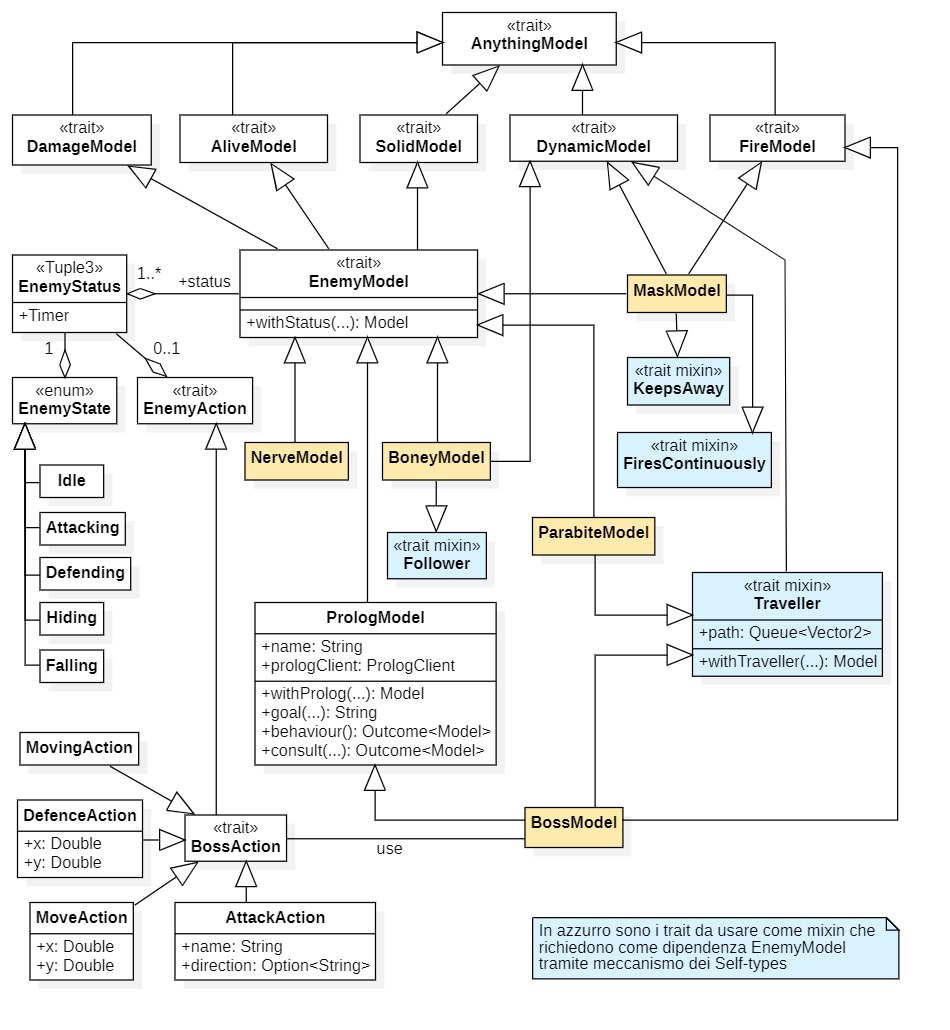
\includegraphics[scale=0.5]{Enemies.jpg}
    \caption{\textit{Gerarchia Enemies}}
\end{figure}

\subsection{AnythingView e AnythingViewModel}

Come scelta di design stabiliamo che 
\begin{itemize}
    \item Una View e un ViewModel devono essere progettati per uno specifico Model. 
    \item Un ViewModel potrebbe essere usato da diverse View
    \item Una View potrebbe non necessitare di un ViewModel: in generale quando non ha animazioni complesse
    \item Un ViewModel viene istanziato con lo stesso identificativo univoco usato per l'oggetto Model a cui si riferisce
    \item Un Model potrebbe disporre di diverse versioni di View ma la sua istanza ne utilizza una
\end{itemize}
Per la View abbiamo pensato di adottare il pattern \textbf{Family Polymorphism} definendo al suo interno i type member astratti \textbf{Model} e \textbf{ViewModel} che vengono concretizzati dai sottotipi della View.
Nella versione finale tuttavia i due tipi interni vengono collegati a dei parametri generici in quanto abbiamo trovato che questa soluzione
\begin{itemize}
    \item ci offre tutti i vantaggi di avere dei type member come la pulizia del codice o la possibilità di usare path-dependent types
    \item ci ha dato meno problemi di type inference 
    \item ci consente di risolvere il problema di type test runtime su tipi astratti \textit{(vedi approfondimento su implementazione)}
    \item a nostro avviso è più espressiva per indicare cosa richiede una View
\end{itemize}

Il pattern \textbf{Family Polymorphism} è stato applicato definendo il tipo astratto \textbf{View} che rappresenta il contenuto grafico da visualizzare attraverso il metodo \textbf{draw}, quest'ultimo richiama il template method \textbf{view} per ottenerlo.

\begin{figure}[!hbt]
    \centering
    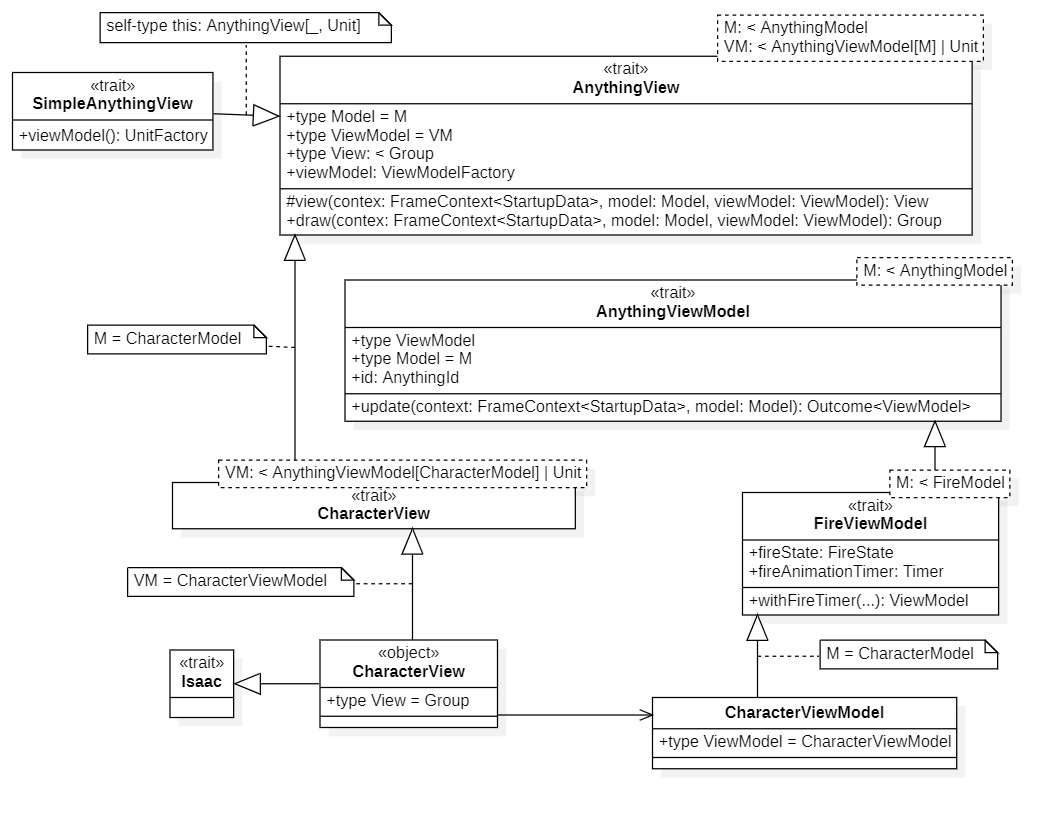
\includegraphics[scale=0.45]{AnythingViewModel.jpg}
    \caption{\textit{Gerarchia AnythingView e AnythingViewModel}} 
\end{figure}

In figura mostriamo l'utilizzo degli \textbf{Union Types} per definire che un ViewModel può non essere richiesto da una View.
Per la gerarchia di ViewModel valgono gli stessi concetti già menzionati per il Model di immutabilità e polimorfismo F-Bounded.
L'esempio concreto di utilizzo in figura riguarda il Character, ma è definito almeno un singleton object View per ciascun Model.

\subsubsection{Asset e animazioni}

\subsection{Sistema di controllo delle collisioni}
Il sistema di controllo delle collisioni ha l'obbiettivo di verificare se due elementi all'interno di una stanza collidono. 
Se questo accade, è necessario aggiornare la posizione degli elementi per evitare che gli elementi si intersechino e gestire un side effect che potrebbe o meno esserci durante la collisione (danno). 

Il sistema agisce e controlla solamente gli Anything di tipo Solid all'interno della stanza correntemente visualizzata.
Essendo il GameModel un'istantanea immutabile, il controllo avviene ad ogni Frame e su una struttura dati statica. 

Il sistema è composto da una serie di funzioni racchiusi in un modulo e sfruttato dal GameModel stesso, il quale va a controllare gli Anything presenti nella Room corrente e ritorna un modello aggiornato, come si può vedere in figura 6.

Il controllo è eseguito in due momenti distinti: 
\begin{enumerate}
  \item In un primo momento viene verificata la collisione tra un elemento e tutti gli altri interni alla stanza. Per ogni collisione viene applicata una funzione all'elemento che corrisponde al side effect.
  \item In un secondo momento vengono ricontrollate le collisioni e spostati gli elementi di conseguenza. 
\end{enumerate}

Il doppio controllo è dovuto al fatto che non è possibile spostare subito un elemento, perchè si potrebbero perdere collisioni con altri elementi.
Questo aspetto, in termini di prestazioni, è largamente migliorabile, ma si rimanda a eventuali sviluppi futuri.


\subsection{Pattern di progettazione}
Di seguito si elencano brevemente i pattern di progettazione utilizzati. 
\subsubsection{Family polimorphism}
Il family polimorphism è stato utilizzato in più di un occasione, tra cui
\begin{itemize}
    \item Definizione di una struttura per il Dungeon, ancora da tipare, ma che già definisce i comportamenti principali di esso.
\end{itemize}
\subsubsection{Bounded F-polimorphism}
\subsubsection{Pimp my library}
Il pattern Pimp my library è stato ampiamente utilizzato, soprattuto per quanto riguarda l'estensione di librerie scritte da terze parti, come ad esempio l'engine Indigo. 
Avendo usato Scala 3 è stato utilizzato il meccanismo degli \textit{extension} method.

In particolare è stata estesa la struttura dati Group di Indigo (rappresentante un gruppo di elementi visualizzabili a schermo), aggiungendo metodi comuni per centrare e scalare gli oggetti in base allo schermo.

Si è sfruttato il pattern anche per modellare le Door come solo struttura dati, per poi modellare i vari comportamenti mediante metodi esterni. Per questa struttura, si è quindi diviso lo stato dal comportamento. 

...andare avanti

\subsubsection{Strategy}
Il pattern strategy è stato utilizzato all'interno della logica di update delle strutture dati. Avendo lavorato con strutture dati immutabili, è stato molto utile definire una funzione comune di aggiornamento che accettasse una strategia di aggiornamento piuttosto che il vero aggiornamento, per via delle logiche a volte innestate che ci si è trovati ad affrontare. 
Un altro momento in cui si è rivelato utile questo pattern è stato all'interno del sistema di gestione delle collisioni, in cui, alla scoperta di una collisione, l'update dell'elemento dipendeva appunto da una strategia variabile. 
\subsubsection{Adapter}
Conversion

\subsection{Organizzazione del codice}
Il codice è stato organizzato in packages. Questi seguono la suddivisione in scene dell'applicativo. Al loro interno, si può ritrovare una suddivisione in Model, View, ViewModel e Componenti.
Il package Core invece, contiene le parti basilari a cui il resto del sistema fa riferimento.

\begin{figure}[!hbt]
    \centering
    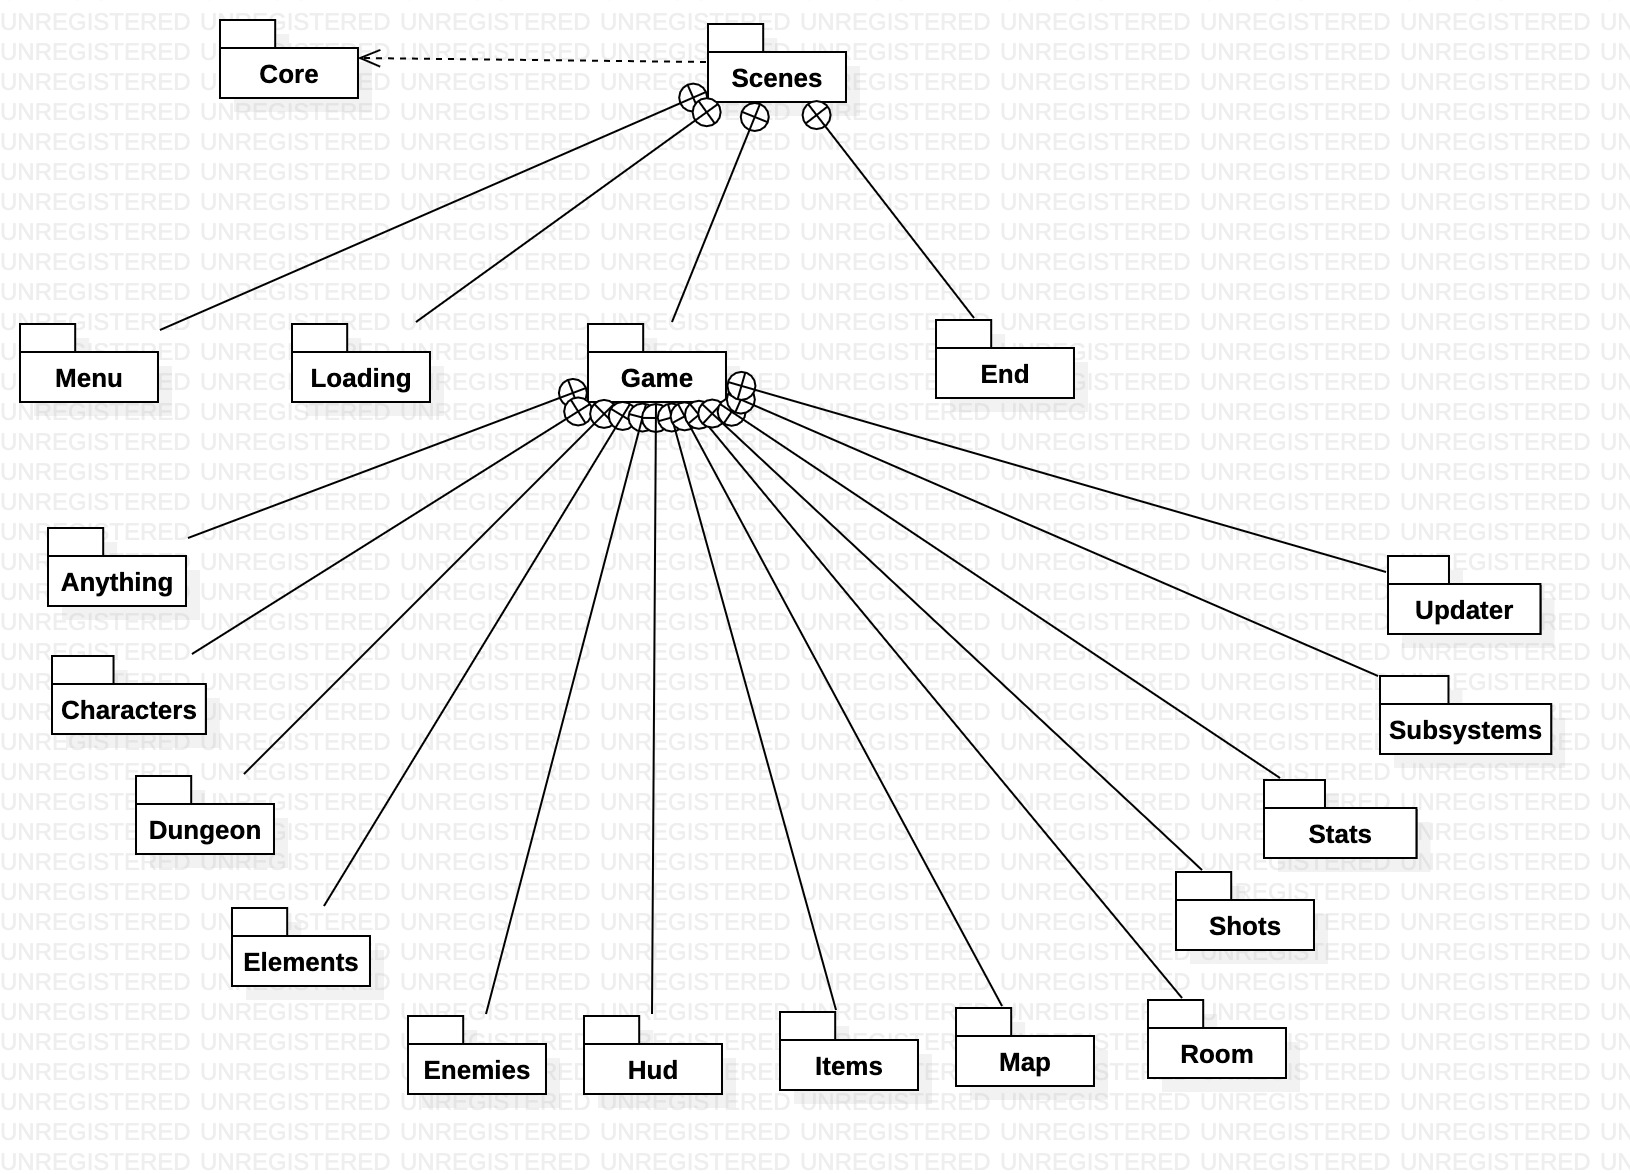
\includegraphics[scale=0.25]{package-diagram.jpg}
    \caption{\textit{Package Diagram del sistema(da modificare con versione pro di staruml)}} 
\end{figure}